\UseRawInputEncoding
\documentclass[reprint, amsmath, amssymb, aps]{revtex4-2}

\usepackage{graphicx}% Include figure files
\usepackage{dcolumn}% Align table columns on decimal point
\usepackage{bm}% bold math
\usepackage{hyperref}% add hypertext capabilities
\usepackage{bibspacing}
\usepackage[font=scriptsize,labelfont=bf, justification=justified]{caption}% change fontsize in captions
\usepackage{float}
\usepackage[english]{babel}
\usepackage{booktabs}% cool table style
\hypersetup{
	colorlinks=true,       % false: boxed links; true: colored links
	linkcolor=black,        % color of internal links
	citecolor=black,        % color of links to bibliography
	filecolor=black,     % color of file links
	urlcolor=black         
}

\begin{document}
	
\title{PHYC30170 Physics with Astronomy and Space Science Lab 1;\\The Brusselator - A Computational Example of Chemical Oscillations}

\author{Daragh Hollman}
\email{daragh.hollman@ucdconnect.ie}
\date{\today}

\begin{abstract}
This report aims to demonstrate and investigate the dynamics of oscillating chemical systems through a study of a specific system known as the Brusselator. This was carried out using Euler's method of numerical integration. It was determined that for ratios of A to B less that 1:2 the system would oscillate but with dampening amplitude until converging to the stable point. Conversely increasing the ratio of A to B resulted in very short periods of dampening before reaching a constant amplitude oscillation. It was also determined that the steady state behaviour of the system was independent of the initial conditions of X and Y as the system converged to the same pattern of constant oscillation regardless of initial conditions with the only difference being in the phase. These findings agree with those found in simulations by Lozno-Parada et al\cite{parada} which exhibits the same steady state behaviour and similarly shows cases where the system converges to the stable point.
\end{abstract}

\maketitle

\section{Introduction}
A chemical oscillator is a non-linear system of reacting chemicals in which exhibits oscillations in the concentrations of their chemicals \cite{nicolis}. Non-linear systems have many applications in modern areas of science and engineering \cite{parada} and find use in non-linear control systems such as periodic drug delivery \citep{oscillationsAdvances}. Due to their complex nature, these kinds of systems can be difficult to set up and maintain as they tend to be very sensitive any changes in their environment conditions. This sensitivity does however does provide some use in the field of analytical chemistry as trace chemicals might upset the oscillatory process \cite{analytical}. The Brusselator is one such system of chemical oscillations and is the focus of this report.

\subsection{Chemical Equations}
Equations describing chemical reactions can be written as follows:
\begin{equation}
	A + B \rightarrow C + D
	\label{eq:chemicalEq}
\end{equation}where chemicals $A$ and $B$ interact with each other to form chemicals $C$ and $D$. This reaction will occur at a specific rate defined by an expression known as a rate equation \cite{dynamics}. It is common to assume that any chemical system will follow mass action kinetics \citep{dynamics}\cite{massAction}, that the reaction rate is direction proportional to the concentration of the reactants. A rate equation for the system in equation \ref{eq:chemicalEq} would look similar to:
\begin{equation}
	-\frac{dA}{dt} = k[A][B]
\end{equation}where $[A]$ and $[B]$ are the concentrations of chemicals A and B respectively and $k$ is the rate constant of the reaction. A negative sign is used to denote that A is decreasing in concentration. In this report we will consider the rate constant to be unity for simplicity.

\subsection{The Brusselator System}
The chemical equations of the Brusselator are typically described as follows \cite{manual}:
\begin{align}
	\begin{aligned}
	A &\rightarrow X & (a)\\
	B + X &\rightarrow Y + D & (b)\\
	2X + Y &\rightarrow 3X & (c)\\
	X &\rightarrow C & (d)
	\end{aligned}
\end{align}

With ODEs given by:
\begin{align}
	\begin{aligned}
	\frac{dX}{dt} &= A - (B + 1)X + X^2 Y & (a)\\
	\frac{dY}{dt} &= BX - X^2 Y & (b)
	\end{aligned}
	\label{eq:rate}
\end{align}

The steady state solution of this system is one which stays stationary over time, sometimes referred to as a stable point. At any stable point, the rate of change of $X$ and $Y$ is zero.
\begin{equation}
	\frac{dX}{dt}=0\,\text{  ;  }\frac{dY}{dt}=0
\end{equation}Hence we can find the stable point by solving for $X$ and $Y$. A full derivation is included in appendix 1, however a single point at $(X, Y) = \left(A, \frac{B}{A}\right)$ was calculated to be the only stable point in the system.\\

In this report we will investigate the evolution of the Brusselator system over time, and discuss the oscillatory nature of the reaction using phase space diagrams and concentration diagrams. This will be carried out over a range of initial conditions for X and Y, but also varying ratios of A and B.

\section{Computational Methods}

\subsection{The Euler Method}
The Euler method was chosen to numerically integrate the rate equations to evolve the system over time. The Euler method is used to solve the first-order initial value problem \cite{eulerError}:
\begin{equation}
	\frac{dy}{dx} = f\left(x, y \right),\, y(x_0) = y_0
\end{equation}Here we have a first-order ordinary differential equation with a known initial condition. Euler's method makes use of a relatively simple process which takes the slope of the function at an initial point and assumes a linear path between that point and the next some arbitrary step away. The formula is given as follows \cite{paulsNotes}:
\begin{equation}
	y(x+h) = y(x) + h f(x, y)
	\label{eq:eulers}
\end{equation}where $h$ is the step size. This will construct the tangent at coordinate $x$, and find the value of $y(x+h)$ to determine the next point. Hence to use Euler's method we can pick a starting point around which we want to approximate and then evaluate equation \ref{eq:eulers} until we have reached the desired number of steps.

\subsubsection{The Application of the Euler method to the System}

The Brusselator system is has two dependent variables which vary with time as shown in the rate equations, see equation \ref{eq:rate}, and hence we need to run two calculations of Euler's method simultaneously. Rewriting these rate equations in the form of equation \ref{eq:eulers}, we have the following:
\begin{align}
	\begin{aligned}
	X_{i+1} &= X_i + \Delta t \frac{dX}{dt} & (a)\\
	Y_{i+1} &= Y_i + \Delta t \frac{dY}{dt} & (b)
	\end{aligned}
	\label{eq:application}
\end{align}where $X_{i}$ is value of $X(t)$ and $X_{i+1}$ is the next step, $X(t+\Delta t)$ with step size $\Delta t$. These variables have the same meaning for equation \ref{eq:application}b but in terms of $Y$.

\subsection{Error Analysis of the Euler Method}
\subsubsection{Round-off Error}
In this simulation two types of error are introduced in the calculations, round-off error and truncation error. Although the round-off error is negligible compared to the truncation error of this simulation, it is important to reference in the context of a computational report. By default Python uses 64 bits to represent a floating point number \cite{python}. One for the sign, 11 for the exponent and 52 for the fraction. This means that we can only accurately represent a maximum of $2^{1024}$ and a minimum of $2^{-1024}$ \cite{niels}. This range is entirely sufficient for the purposes of this report and hence any errors due to round-off are negligible.

\subsubsection{Truncation Error}
Aside from the round-off error there exists a truncation error between the exact solution and the solution estimated by Euler's method. There is the local error between each step and the global error which is the summation of all the local errors up to a certain step \cite{owkes}. If we take the Taylor series approximation for a function:
\begin{equation}
	y_{i+1} = y_{i} + y'_{i}h + \frac{y''_i}{2} h^2 + \dots + \frac{y_i^{(n)}}{n!} h^n + \dots
\end{equation}we can clearly see that the first two terms of this are the same as Euler's method shown in equation \ref{eq:eulers}. The Taylor series will be an exact solution if all terms are included however if we truncate it after the first two terms, what remains will be the difference between Euler's method and the exact solution over a step. This is the local error, and for an ODE with:
\begin{align*}
	\begin{aligned}
	\frac{dy}{dx} &= f(x,y)\\
	y' &= f(x,y)
	\end{aligned}
\end{align*}we have:
\begin{equation}
	y_{i+1} = \underbrace{y_i + f(x_i, y_i) h}_\text{Euler's Method} + \underbrace{\frac{f'(x_i,y_i)}{2}h^2 + \dots}_\text{Error}
\end{equation}We can assume that, with a small step size $h$, that higher order terms will be small. Hence we can take the local error to scale with $\mathcal{O}(h^2)$ and that terms of $\mathcal{O}(h^3)$ or higher are negligible.\\

The global error is the summation of the local errors for each step. As the step size decreases, the number of steps within a length L increases with $h^{-1}$. Hence the global error is given by the following:
\begin{equation}
	\epsilon_g = \frac{1}{h} \sum \epsilon_l
\end{equation}and as the local error scales with $h^2$ and the global error scales with the local error and $h^{-1}$. The global error on the system for any number of steps scales with $\mathcal{O}(h)$, the step size.

\section{Results and Discussion}
Two kinds of plots were created, one showing directly how the concentrations of X and Y vary over time, and the other was a phase space plot of the entire evolution. Chemicals A and B were kept at constant values throughout the evolution while chemicals X and Y were free to vary. Chemical A was given a value of 1 as the concentration of the chemicals is in arbitrary units it made sense to solely vary the concentration of B and inspect different ratios of A to B. For an initial phase space position of $(X, Y) = (0, 0)$, we looked at ratios of A:B of 1:1.5, 1:1.9, 1:2, 1:2.5, and 1:4. These were simulated and plotted in figures \ref{fig:oneToOne-Five}, \ref{fig:oneToOne-Nine}, \ref{fig:oneToTwo}, \ref{fig:oneToTwo-Five}, and \ref{fig:oneToFour} respectively.\\

From these simulations, it was determined that there is a limit on the ratio of A and B to whether the oscillations dampen. We found that a ratio of A:B of less than 1:2 results in continued dampening of the oscillations of chemicals X and Y until arriving at the stable point. This can be seen clearly in figures \ref{fig:oneToOne-Five} and \ref{fig:oneToOne-Nine}. When $B=1.5$ we see rapid dampening with X and Y reaching constant values after 30 seconds, whereas closer to a ratio of 1:2, when $B=1.9$ we see longer oscillations with X and Y only reaching constant values after 100 seconds. This is contrasted by figure \ref{fig:oneToTwo} where A:B is equal to 1:2 and recurring oscillations are present.\\

\begin{figure*}
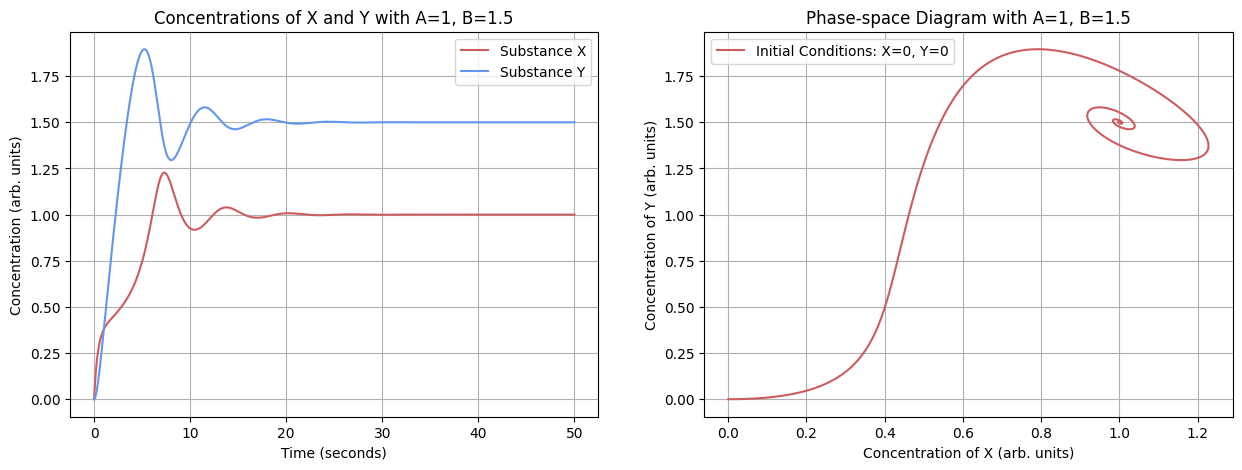
\includegraphics[width=1.65\columnwidth]{combinedPlot_fallToStable.png}
\caption{\label{fig:oneToOne-Five}Evolutions of the system for 50 seconds ($50,000$ steps with a size of $10^{-3}$) with $B=1.5$ and initial conditions $X=0$, $Y=0$. \textbf{Left:} Concentration of each chemical over time. We see a damping in the oscillations as the system falls towards the stable point of the system. \textbf{Right:} A phase space plot of the evolution of the concentrations of X and Y over time. We can visually see the damping of the oscillations as the system evolves and stops on the stable point (1, 1.5).}
\end{figure*}

\begin{figure*}
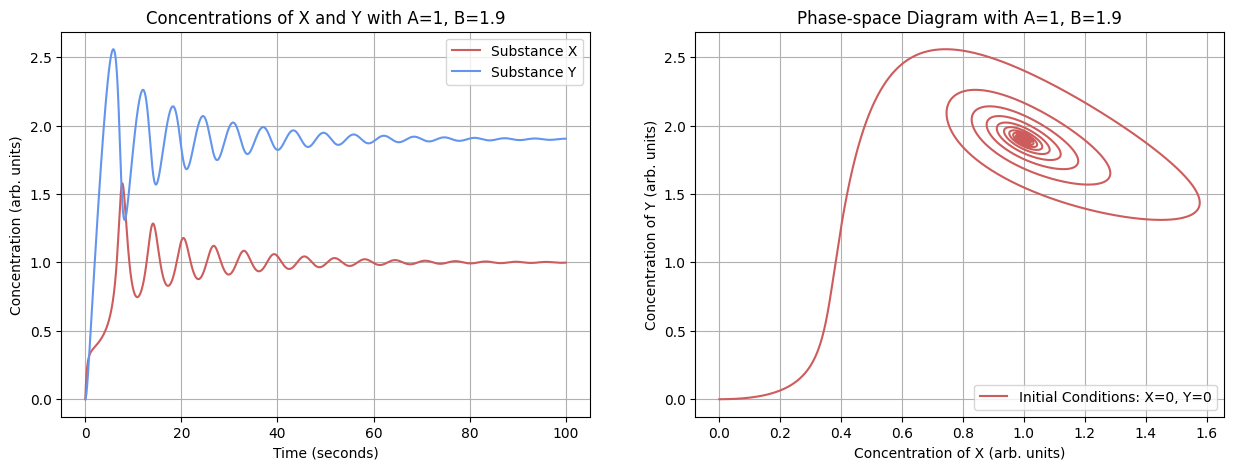
\includegraphics[width=1.65\columnwidth]{oneToOne-Nine.png}
\caption{\label{fig:oneToOne-Nine}Evolutions of the system for 100 seconds ($100,000$ steps with a size of $10^{-3}$) with $B=1.9$ and initial conditions $X=0$, $Y=0$. Similarly to figure \ref{fig:oneToOne-Five} we see dampening before converging on the stable point.}
\end{figure*}

\begin{figure*}
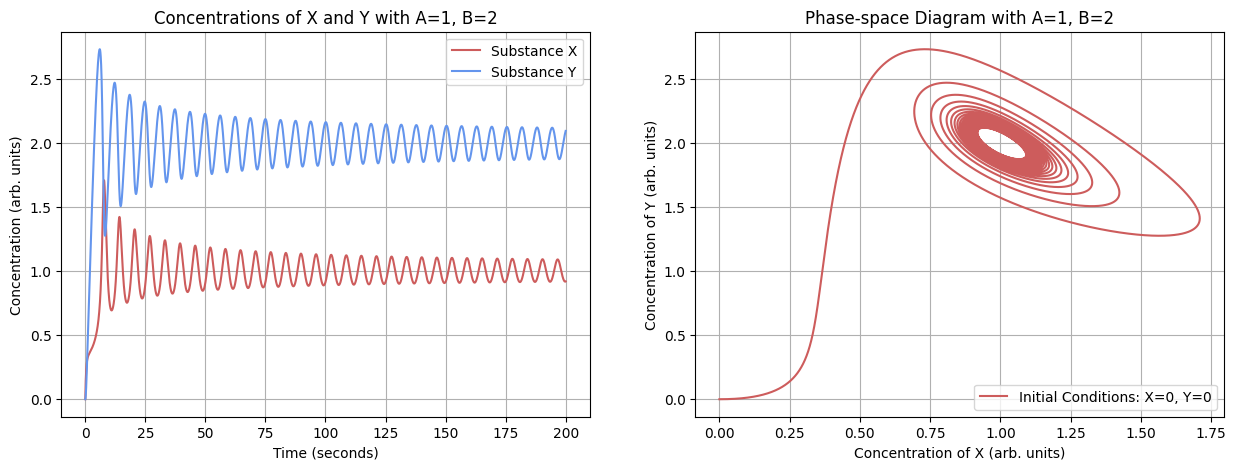
\includegraphics[width=1.65\columnwidth]{combinedPlot.png}
\caption{\label{fig:oneToTwo}Evolutions of the system for 200 seconds ($200,000$ steps with a size of $10^{-3}$) with $B=2$ and initial conditions $X=0$, $Y=0$. \textbf{Left:} Concentration of each chemical over time. The oscillations in the concentration of each chemical can be clearly seen. \textbf{Right:} A phase space plot of the evolution of the concentrations of X and Y over time. We can see the amplitude of the oscillations decreases before reaching a stable constant amplitude. The oscillations are around the stable point (1, 2).}
\end{figure*}

For higher ratios of A:B, such as in figures \ref{fig:oneToTwo-Five} and \ref{fig:oneToFour} we still see consistent oscillations however we also see much larger amplitude oscillations for increasing ratios. It can also be seen that the concentrations approach their constant amplitude much quicker meaning the damping time is shorter. The simulation in figure \ref{fig:oneToTwo-Five} reaches constant amplitude in less than 20 seconds and the simulation in figure \ref{fig:oneToFour} reaches constant amplitude almost immediately (less than 10 seconds). This is contrasted by figure \ref{fig:oneToTwo} where the oscillations reach constant amplitude after approximately 150 seconds. \\

\begin{figure*}
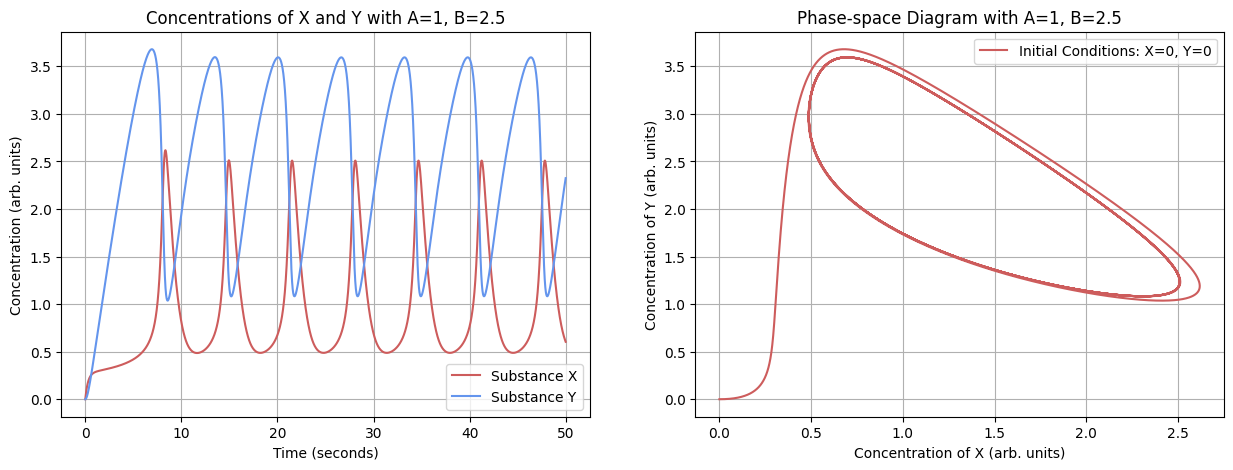
\includegraphics[width=1.65\columnwidth]{oneToTwo-Five.png}
\caption{\label{fig:oneToTwo-Five}Evolutions of the system for 50 seconds ($50,000$ steps with a size of $10^{-3}$) with $B=2.5$ and initial conditions $X=0$, $Y=0$. Here we see that a larger ratio of A:B results in a quicker approach to constant amplitude oscillations.}
\end{figure*}

\begin{figure*}
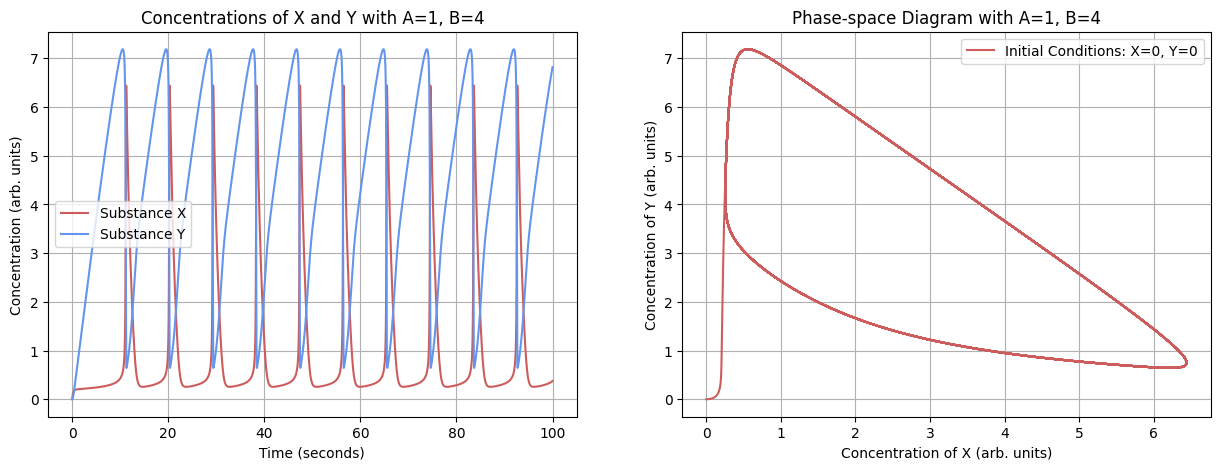
\includegraphics[width=1.65\columnwidth]{oneToFour.png}
\caption{\label{fig:oneToFour}Evolutions of the system for 100 seconds ($100,000$ steps with a size of $10^{-3}$) with $B=4$ and initial conditions $X=0$, $Y=0$. Again we see that a larger ratio of A:B results in a quicker approach to constant amplitude oscillations. We also see much larger amplitude oscillations due to the increase in the constant supply of chemical B.}
\end{figure*}

Figure \ref{fig:multiPlot} shows the effect of the initial conditions of X and Y on the oscillations. It can be clearly seen from the phase space plot that the steady state behaviour is independent of the initial conditions of X and Y. It can be seen that regardless of initial location on the phase space plot, each path dampens towards the same constant path in phase space of constant amplitude oscillations. This is demonstrated too by the second plot in figure \ref{fig:multiPlot}. Despite each line of concentration being out of phase with one another, it can clearly be seen that they follow the same pattern of oscillations, dampening at the same rate until reaching a constant amplitude.

\begin{figure}
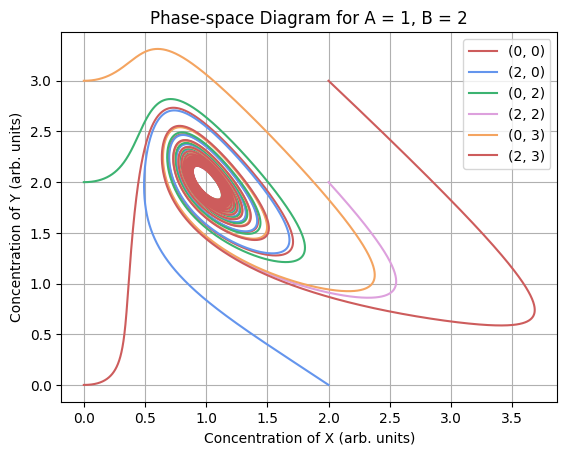
\includegraphics[width=0.85\columnwidth]{variationOfInitialConditions_phase.png}
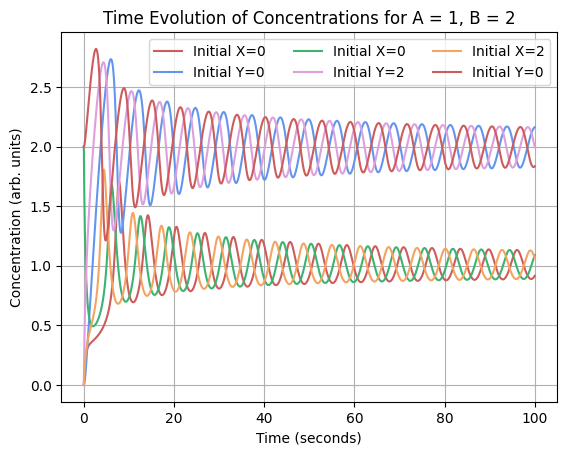
\includegraphics[width=0.85\columnwidth]{variationOfInitialConditions_evolution.png}
\caption{\label{fig:multiPlot}Plots showing the differences between 6 different initial conditions for $B=2$. We see all initial conditions yield the same steady state behaviour. The upper plot shows that each system dampens before reaching the same steady amplitude oscillation surrounding the stable point at (1,2). Although in the lower plot we see each system is out of phase with each other, we see that they still all track the same shape showing an equal dampening regardless of their initial conditions.}
\end{figure} 

\section{Conclusion}
The aim of this report was to demonstrate and investigate, using Euler's numerical method, the dynamics of the Brusselator system as an example of oscillating chemical reactions. The system was looked at with varying initial constants A and B, along with varying initial conditions of the chemicals being investigated X and Y. It was determined that for ratios of A to B less that 1:2 the system would oscillate but with dampening amplitude until converging to the stable point. Conversely increasing the ratio of A to B resulted in very short periods of dampening before reaching a constant amplitude oscillation. It was also determined that the steady state behaviour of the system was independent of the initial conditions of X and Y as the system converged to the same pattern of constant oscillation regardless of initial conditions with the only difference being in the phase. These findings agree with those found in simulations by Lozno-Parada et al\cite{parada} which exhibits the same steady state behaviour and similarly shows cases where the system converges to the stable point.

\clearpage
\bibliography{chemOscillationsReferences.bib}

\clearpage

\section*{Appendix 1 - Derrivation of the Stable Point}
\begin{align*}
	\begin{aligned}
	A - (B + 1)X + X^2 Y &= 0\\
	BX - X^2 Y &= 0\\
	\\
	\therefore \hspace{1cm} X^2 Y &= BX\\
	\\
	\implies A - (B + 1)X + BX &= 0\\
	X &= A\\
	\\
	A^2 Y &= BA\\
	\implies Y &= \frac{B}{A}\\
	\\
	(X, Y) &= \left(A, \frac{B}{A}\right)
	\end{aligned}
\end{align*}

\end{document}



